\documentclass[../../main.tex]{subfiles}
\begin{document}
Sweep Line is a type of algorithm that mainly used to solve problems with intervals of one-dimensional. Let us look at one example:
1. 253. Meeting Rooms II

Given an array of meeting time intervals consisting of start and end times [[s1,e1],[s2,e2],...] (si < ei), find the minimum number of conference rooms required.
\begin{lstlisting}
Example 1:

Input: [[0, 30],[5, 10],[15, 20]]
Output: 2

Example 2:

Input: [[7,10],[2,4]]
Output: 1
\end{lstlisting}
It would help a lot if at first we can draw one example with cooridinates.
\begin{figure}[h]
    \centering
    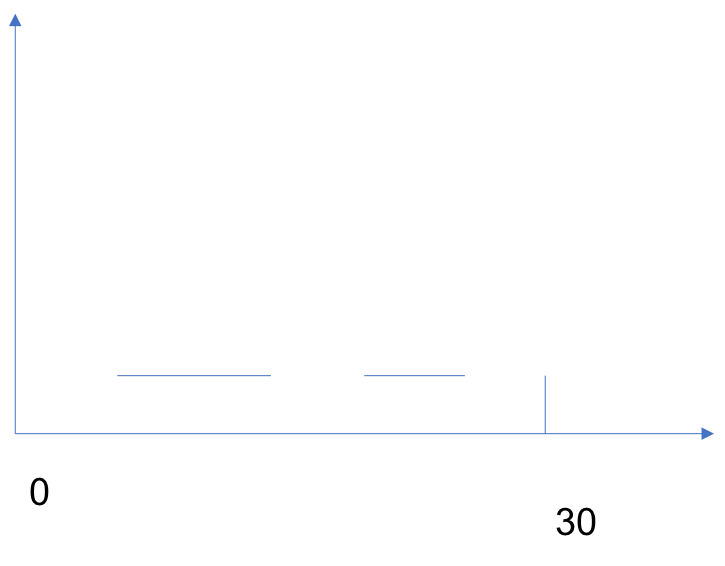
\includegraphics[width = 0.6\columnwidth]{fig/sweep_line_253.png}
    \caption{Interval questions}
    \label{fig:interval}
\end{figure}
First, the simplest situation is when we only need one meeting room is there is no intersection between these time intervals. If we add one interval that only intersect with one of the previous intervals, this means we need two conference rooms. So to find the minimum conference rooms we need, we need to find the maximum number of intersection between these time intervals. The most native solution is to scan all the time slot in one for loop, and at another inner loop go through all the intervals, if this time slot is in this intervals, then we increase the minimum number of meeting room counter. This gives us time complexity of $O(n*m)$, where $n$ is the number of intervals and $m$ is the total number of time slots. The Python code is as follows, unfortunately, with this solution we have LTE error.  
\begin{lstlisting}[language = Python]
# Definition for an interval.
# class Interval(object):
#     def __init__(self, s=0, e=0):
#         self.start = s
#         self.end = e

from collections import defaultdict
from heapq import heappush, heappop
from sys import maxint
class Solution(object):
    def minMeetingRooms(self, intervals):
        """
        :type intervals: List[Interval]
        :rtype: int
        """
        if not intervals:
            return 0
        #solution 1, voting, time complexity is O(e1-s1), 71/77 test, TLE
        votes = defaultdict(int)
        num_rooms = 0   
        for interval in intervals:
            s=interval.start
            e=interval.end
            for i in range(s+1,e+1):
                votes[i]+=1
                num_rooms = max(num_rooms, votes[i])
        return num_rooms
\end{lstlisting}
\subsection{Speedup with Sweep Line}
Now, let us see how to speed up this process. We can use Sweep Line method. For the sweep line, we have three basic implementations: one-dimensional, min-heap, or map based. 
\subsubsection{One-dimensional Implementation}
 To get the maximum number of intersection of all the intervals, it is not necessarily to scan all the time slots, how about just scan the key slot: the starts and ends . Thus, what we can do is to open an array and put all the start or end slot into the array, and with $1$ to mark it as start and $0$ to mark it as end. Then we sort this array. Till this point, how to get the maximum intersection? We go through this sorted array, if we get a start our current number of room needed will increase by one, otherwise, if we encounter an end slot, it means one meeting room is freed, thus we decrease the current on-going meeting room by one. We use another global variable to track the maximum number of rooms needed in this whole process. Great, because now our time complexity is decided by the number of slots $2n$, with the sorting algorithm, which makes the whole time complexity $O(nlogn)$ and space complexity $n$. This speeded up algorithm is called Sweep Line algorithm. Before we write our code, we better check the \textit{special cases}, what if there is one slot that is marked as start in one interval but is the end of another interval. This means we can not increase the counting at first, but we need to decrease, so that the sorting should be based on the first element of the tuple, and followed by the second element of the tuple. For example, the simple case $[[13,15],[1,13]]$, we only need maximum of one meeting room. Thus it can be implemented as:
\begin{figure}[h]
    \centering
    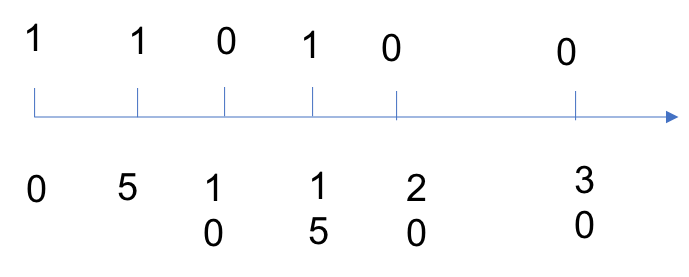
\includegraphics[width=0.6\columnwidth]{fig/sweep_line_one_dimension.png}
    \caption{One-dimensional Sweep Line}
    \label{fig:one_dim_sl}
\end{figure}
\begin{lstlisting}[language=Python]
 def minMeetingRooms(self, intervals):
        if not intervals:
            return 0       
        #solution 2
        slots = []
        # put slots into one-dimensional axis
        for i in intervals:
            slots.append((i.start, 1))
            slots.append((i.end, 0))
        # sort these slots on this dimension
        #slots.sort(key = lambda x: (x[0], x[1]))
        slots.sort()
        
        # now execute the counting
        crt_room, max_room = 0, 0
        for s in slots:
            if s[1]==0: # if it ends, decrease
                crt_room-=1
            else:
                crt_room+=1
            max_room = max(max_room, crt_room)
        return max_room
\end{lstlisting}
\subsubsection{Min-heap Implementation}
\begin{figure}[h]
    \centering
    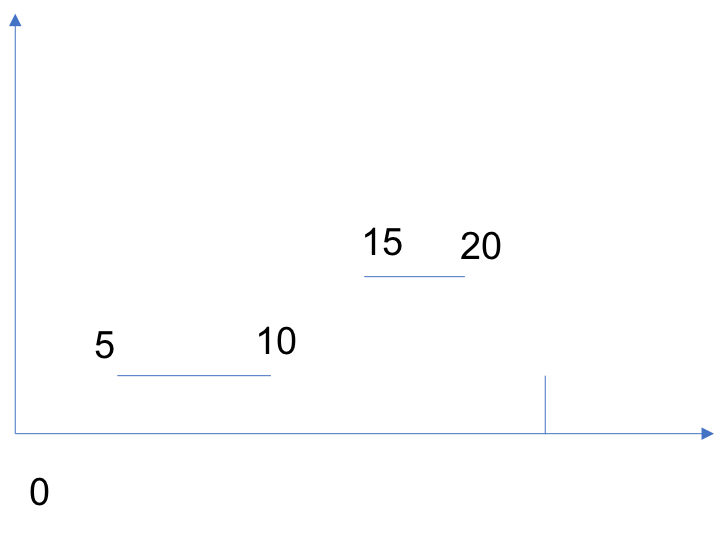
\includegraphics[width=0.6\columnwidth]{fig/sweep_line_min_heap.png}
    \caption{Min-heap for Sweep Line}
    \label{fig:min_heap_sl}
\end{figure}
Instead of opening an array to save all the time slots, we can directly sort the intervals in the order of the start time. We can see Fig.~\ref{fig:min_heap_sl}, we go through the intervals and visit their end time, the first one we encounter is $30$, we put it in a min-heap, and then we visit the next interval $[5, 10]$, $5$ is smaller than the previous end time $30$, it means this interval intersected with a previous interval, so the number of maximum rooms increase $1$, we get $2$ rooms now. We put $10$ into the min-heap. Next, we visit $[15, 20]$, $15$ is larger than the first element in the min-heap $10$, it means that these two intervals can be merged into one $[5, 20]$, so we need to update the end time $10$ to $20$. 

This way, the time complexity is still the same which is decided by the sorting algorithm. While the space complexity is decided by real situation, it varies from $O(1)$ (no intersection) to $O(n)$ (all the meetings are intersected at at least one time slot).  
\begin{lstlisting}[language=Python]
def minMeetingRooms(self, intervals):
        if not intervals:
            return 0
        #solution 2
        intervals.sort(key=lambda x:x.start)
        h = [intervals[0].end]
        rooms = 1
        for i in intervals[1:]:
            s,e=i.start, i.end
            e_before = h[0]
            if s<e_before: #overlap
                heappush(h, i.end)
                rooms+=1
            else: #no overlap
                #merge
                heappop(h) #kick out 10 in our example
                heappush(h,e) # replace 10 with 20
        return rooms
\end{lstlisting}
% 2、multiset:这次是先对每个区间的起点排序,然后依次将每个区间的终点放在一个集合中。如果下一个区间的起点大于等于之前某个区间的终点,就将其从集合中删除,每次需要统计一下当前所需的最大办公室数量。这个版本的时间复杂度还是O(nlogn),但是空间复杂度却变成output-dependent的了,最多是O(n),最少是O(1)。
\subsubsection{Map-based Implementation}

% 3、map:我们用一个map来存储重合区域,即每个区间的起点代表一个区间的开始,会将重叠区域+1,每个区间的结束点代表一个区间的结束,会将重叠区域-1。因此我们可以利用这个性质,结合STL中的map来实现(实质上这个算法和“一维向量”版本非常像,只是采用的数据结构不同而已)。
% --------------------- 
% 作者:魔豆Magicbean 
% 来源:CSDN 
% 原文:https://blog.csdn.net/magicbean2/article/details/74199529 
% 版权声明:本文为博主原创文章,转载请附上博文链接!

\begin{lstlisting}[language=Python]
class Solution {
public:
    int minMeetingRooms(vector<Interval>& intervals) {
        map<int, int> mp;
        for (auto val : intervals) {
            ++mp[val.start];
            --mp[val.end];
        }
        int max_room = 0, crt_room = 0;
        for (auto val : mp) {
            crt_room += val.second;
            max_room = max(max_room, crt_room);
        }
        return max_room;
    }
};
\end{lstlisting}

\subsection{LeetCode Problems}
\begin{enumerate}
 \item \textbf{986. Interval List Intersections} Given two lists of closed intervals, each list of intervals is pairwise disjoint and in sorted order. Return the intersection of these two interval lists.
\begin{lstlisting}[numbers=none]
Input: A = [[0,2],[5,10],[13,23],[24,25]], B = [[1,5],[8,12],[15,24],[25,26]]
Output: [[1,2],[5,5],[8,10],[15,23],[24,24],[25,25]]
Reminder: The inputs and the desired output are lists of Interval objects, and not arrays or lists.
\end{lstlisting}
\end{enumerate}

\end{document}